\chapter{Vergleich der Einkommensverteilungen anhand mehrerer Indikatoren}

Im Folgenden soll die Einkommensverteilung in Deutschland mit der weltweiten Einkommensverteilung anhand mehrerer Indikatoren verglichen werden. Die Indizes, die hierfür verwendet werden, sind das Verhältnis des Durchschnittseinkommens der reichsten 10\% zum Durchschnittseinkommens der ärmsten 50\%, der Gini-Koeffizient und der Bevölkerungsanteil mit einem Einkommen unterhalb der Armutsgrenze. Durch die Auswertung dieser Kennzahlen soll ein umfassendes Verständnis über die Einkommensverteilung Deutschlands im weltweiten Vergleich geschaffen werden.
\section{T10/ B50 Einkommensverhältnis}

Zuerst wird das gewichtete Verhältnis des Einkommensanteils der reichsten 10\% zum Einkommensanteil der ärmsten 50\% betrachtet (Im Folgenden als ''T10/B50'' abgekürzt). Es gibt an, wie hoch der Anteil der reichsten 10\% am Gesamteinkommen im Vergleich zu den ärmsten 50\% gewichtet nach der absoluten Grö{\ss}e der Gruppen ist. Je höher der Wert, desto ungleicher sind die Einkommen verteilt. \footcite[Vgl.][S. 31]{wir_2022}

\begin{figure}[H]
    \centering
    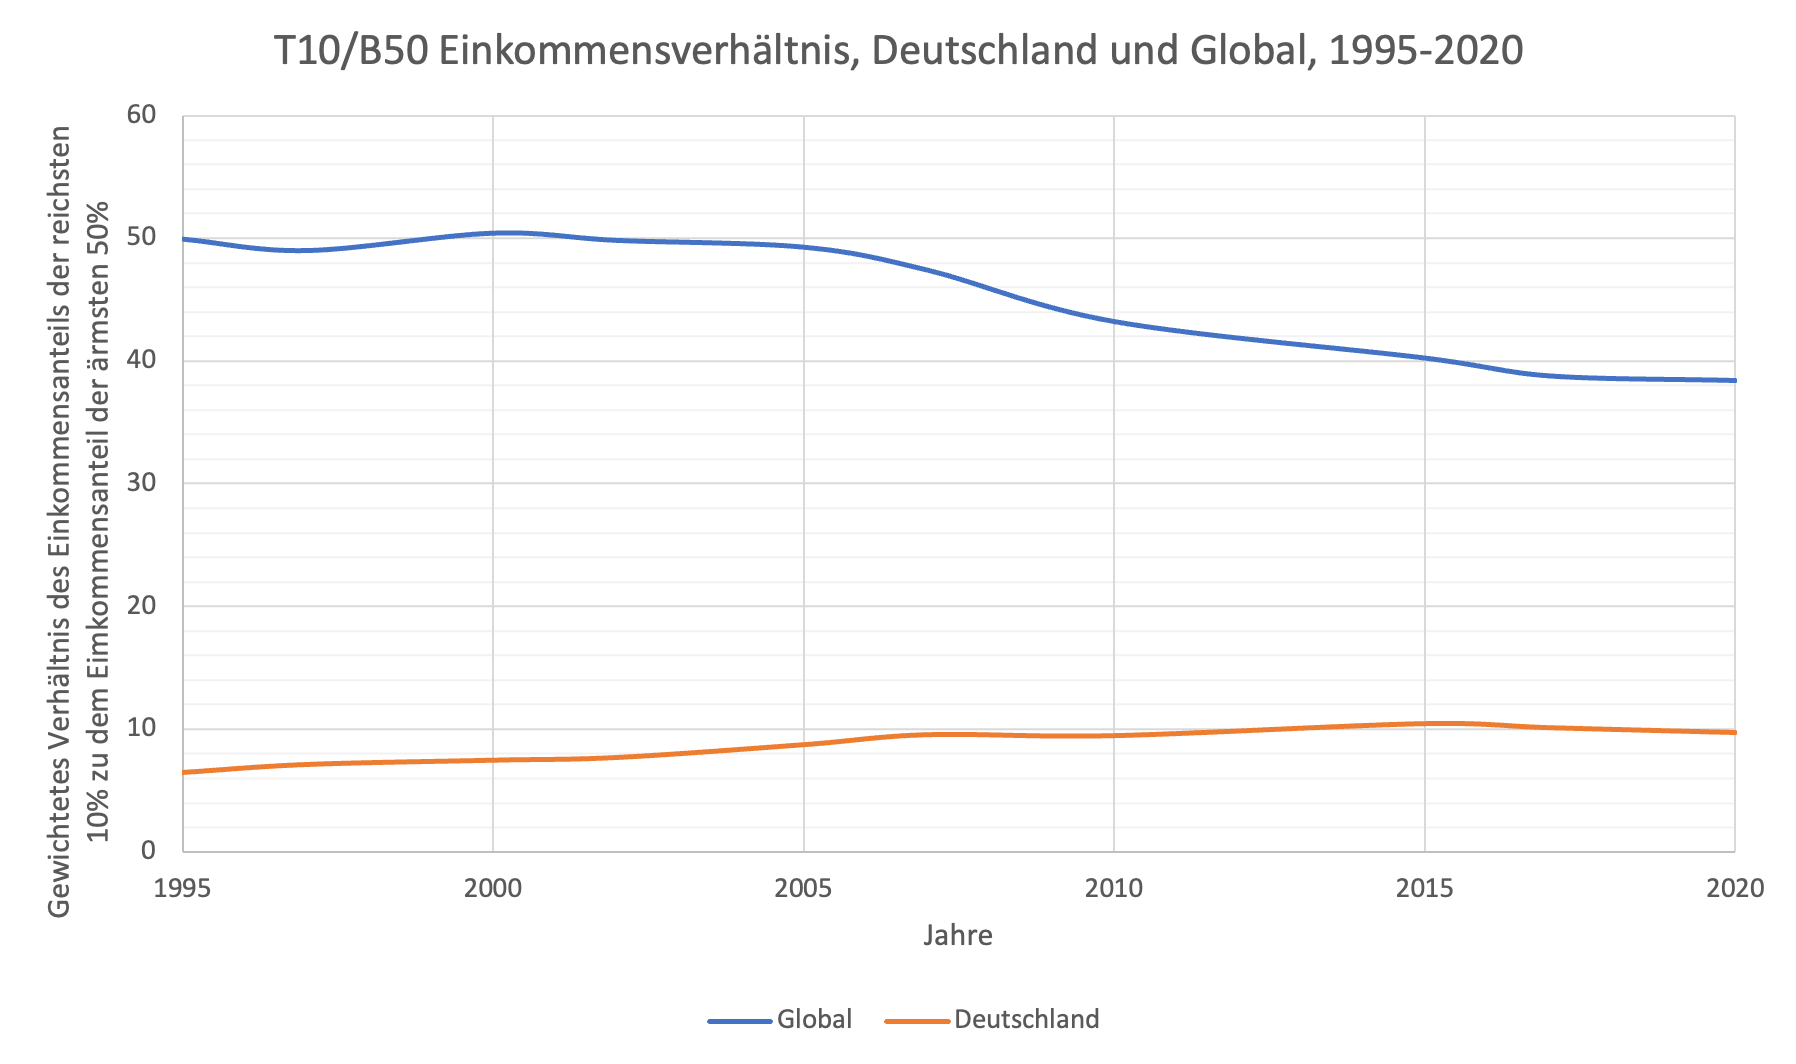
\includegraphics[height=8.15cm]{Bilder/T10B50-Ratio3.png}
    \caption[T10/B50 Einkommensverhältnis, Deutschland und global, 1995-2020]{gewichtetes Verhältnis des Einkommensanteils der reichsten 10\% zum Einkommensanteil der ärmsten 50\% in Deutschland und auf globaler Ebene von 1995 bis 2020. Eigene Darstellung und Berechnung. Daten abgerufen von \cite[][, S.55, 195]{wir_2022} am 01.03.2024.}
    \label{fig:iso_norm}
\end{figure}

Anhand der Grafik ist zu erkennen, dass das T10/B50-Verhältnis in Deutschland von 1995 bis 2015 von ca. 6 auf 10 stetig angestiegen ist.  Seit 2015 ist das Verhältnis eher konstant geblieben. Somit müssen die Einkommen des obersten Dezils von 1995 bis 2015 stärker gestiegen sein als die Einkommen der unteren Hälfte der Bevölkerung. Nach Daten des DIW sind die Realeinkommen des obersten Dezils in diesem Zeitraum um fast 30\% gestiegen, während die Einkommen der unteren Hälfte nur um ca. 10\% gestiegen sind. \footcite[Vgl.][S. 452]{grabka_einkommensverteilung_2018} Ein möglicher Grund für diese Entwicklung sind unter anderem die gestiegene Arbeitslosigkeit von 2000 bis 2005 sein, für eine Lohnzurückhaltung gesorgt und die unteren Einkommen stärker getroffen hat. Als weiteren Grund ist die ab 2007 deutlich verstärkte Zuwanderung. Diese neu zugezogenen Menschen brauchen meist mehr Zeit um sich am Arbeitsmarkt zu etablieren und nehmen im Durchschnitt eher niedrigerer entlohnte Arbeitsstellen an. Als weitere untergeordnete Ursachen für den Anstieg des T10/B50-Verhältnisses können noch eine Ausweitung des Niedriglohnsektors und eine sub-inflationäre Entwicklung der Sozialleistungen bis 2015 genannt werden. \footcite[Vgl.][S. 453f]{grabka_einkommensverteilung_2018}

Im Gegensatz dazu ist der Indikator auf globaler Ebene im Betrachtungszeitraum von 1995 bis 2005 eher seitwärts entwickelt und ist dann ab 2005 fast konstant von ca. 50 auf 38 gefallen. Dieser Abfall könnte durch die Finanzkrise 2008 und die daraus resultierenden wirtschaftlichen Veränderungen verursacht worden sein. \footcite[Vgl.][S. 55]{wir_2022}

Insgesamt ist festzustellen, dass das T10/B50-Verhältnis in Deutschland im Vergleich zu dem globalen Wert deutlich niedriger ist. Diese Diskrepanz ist kann durch die in Europa hohen bzw. in Deutschland noch höheren Umverteilungsraten begründet werden. \footcite[Vgl.][S. 36f]{wir_2022} Dennoch hat sich der Abstand zwischen Deutschland und dem globalen Wert in den letzten 25 Jahren von ca. 44 auf 28 verringert, was größtenteils auf einen Rückgang des Indikators auf globaler Ebene, jedoch auch auf einen Anstieg des Indikators in Deutschland zurückzuführen ist. Zusammenfassend lässt sich sagen, dass sich die Einkommensverteilungen in Deutschland und auf globaler Ebene in den letzten 25 Jahren angenährt haben, Deutschland aber immernoch eine deutlich geringere Einkommensungleichheit aufweist.

\section{Gini-Koeffizient}

Der zweite herangezogene Indikator ist der Gini-Koeffizient. Er ist ein Ma{\ss} für die (Un-)Gleichverteilung von Einkommen und Vermögen. Er kann Werte zwischen 0 und 1 annehmen, wobei 0 für eine vollkommene Gleichverteilung und 1 für eine vollkommene Ungleichverteilung steht. \footcite[Vgl.][]{gini_definition_diw_2024}

\begin{figure}[H]
    \centering
    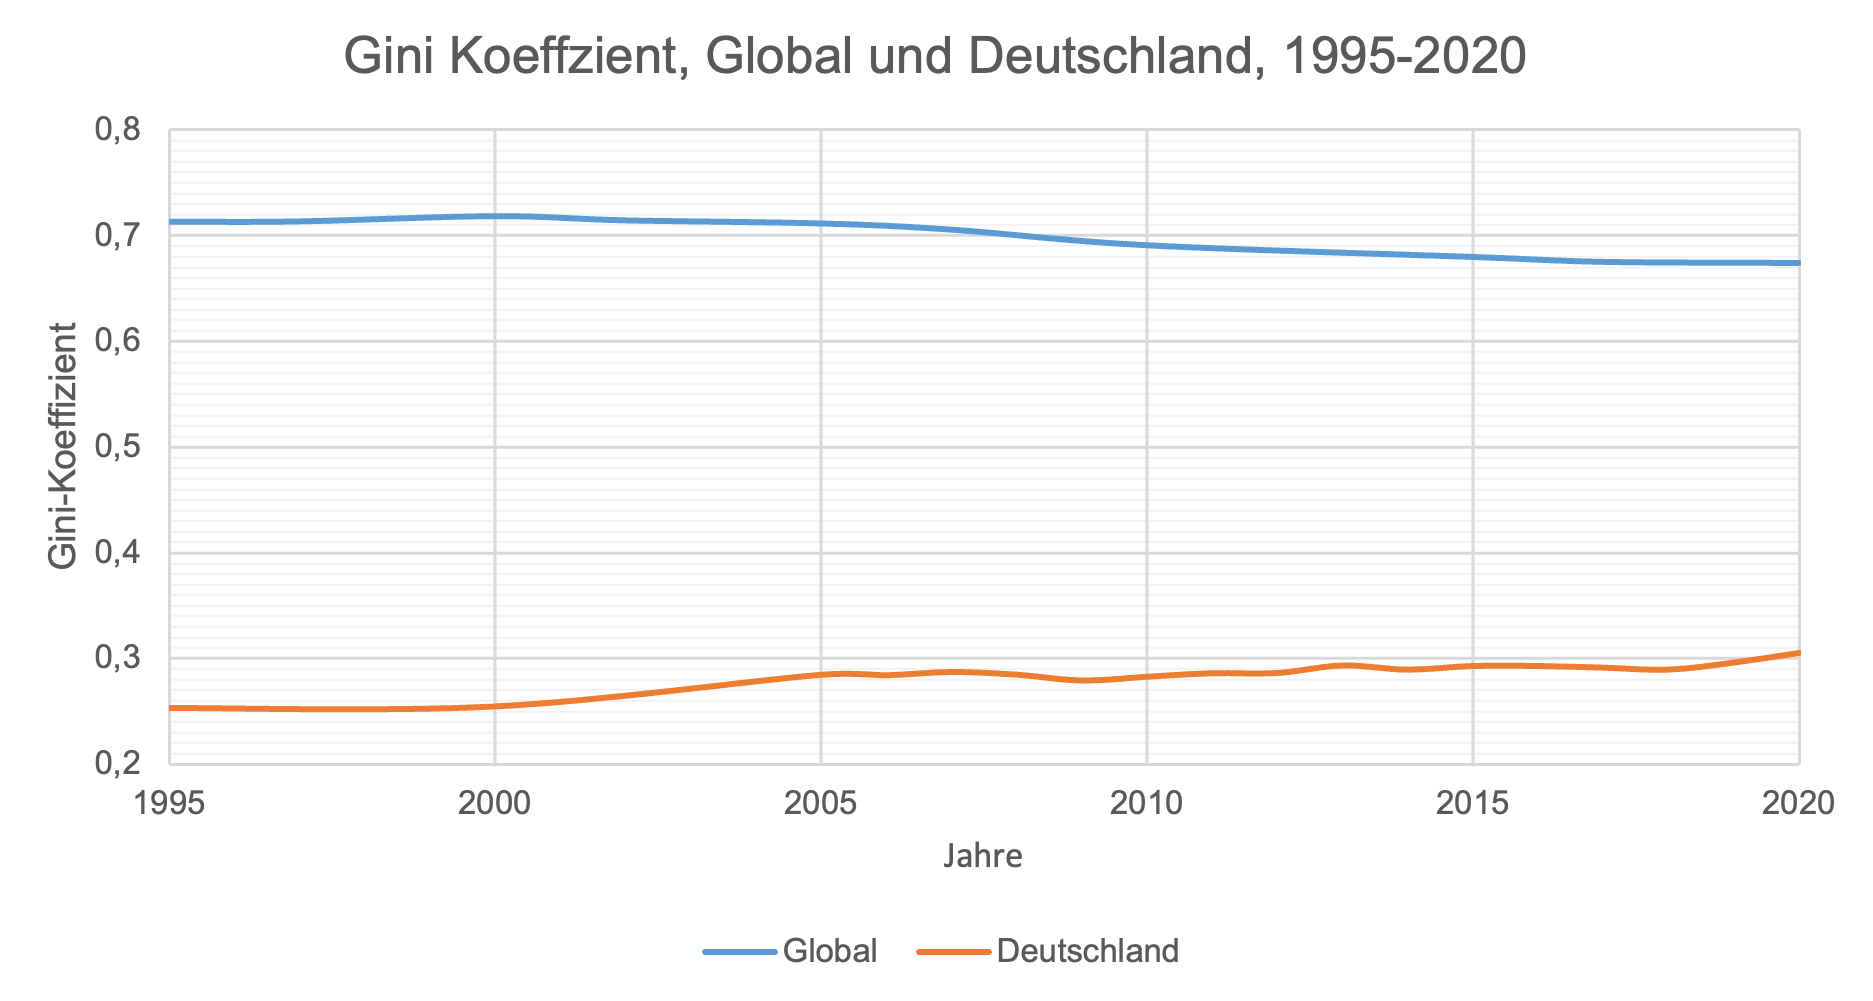
\includegraphics[height=8cm]{Bilder/Gini-Koeffizient2.png}
    \caption[Gini-Koeffizient, Deutschland und global, 1995-2020]{Gini-Koeffizient für Deutschland und auf globaler Ebene von 1995 bis 2020. Eigene Darstellung. Daten abgerufen von \cite[][, S.56 (global)]{wir_2022} und \cite[][(Deutschland)]{bmas_arb_gini_2020} am 01.03.2024.}
    \label{fig:iso_norm}
\end{figure}

\section{Bevölkerungsanteil unterhalb der Armutsgrenze}

Als letzte Kennzahl wird der Anteil der Bevölkerung mit einem Einkommen unterhalb der Armutsgrenze betrachtet. In Deutschland ist die Armutsrisikoquote bei 60\% des Medianeinkommens angesetzt. \footcite[Vgl.][]{bmas_arb_armutsrisikoquote_2023} Für die globale Betrachtung werden die jeweiligen Einkommensgrenzen, die jedes Land für sich definiert hat, verwendet. \footcite[Vgl.][]{wb_armutsquote_global_2022}

\begin{figure}[H]
    \centering
    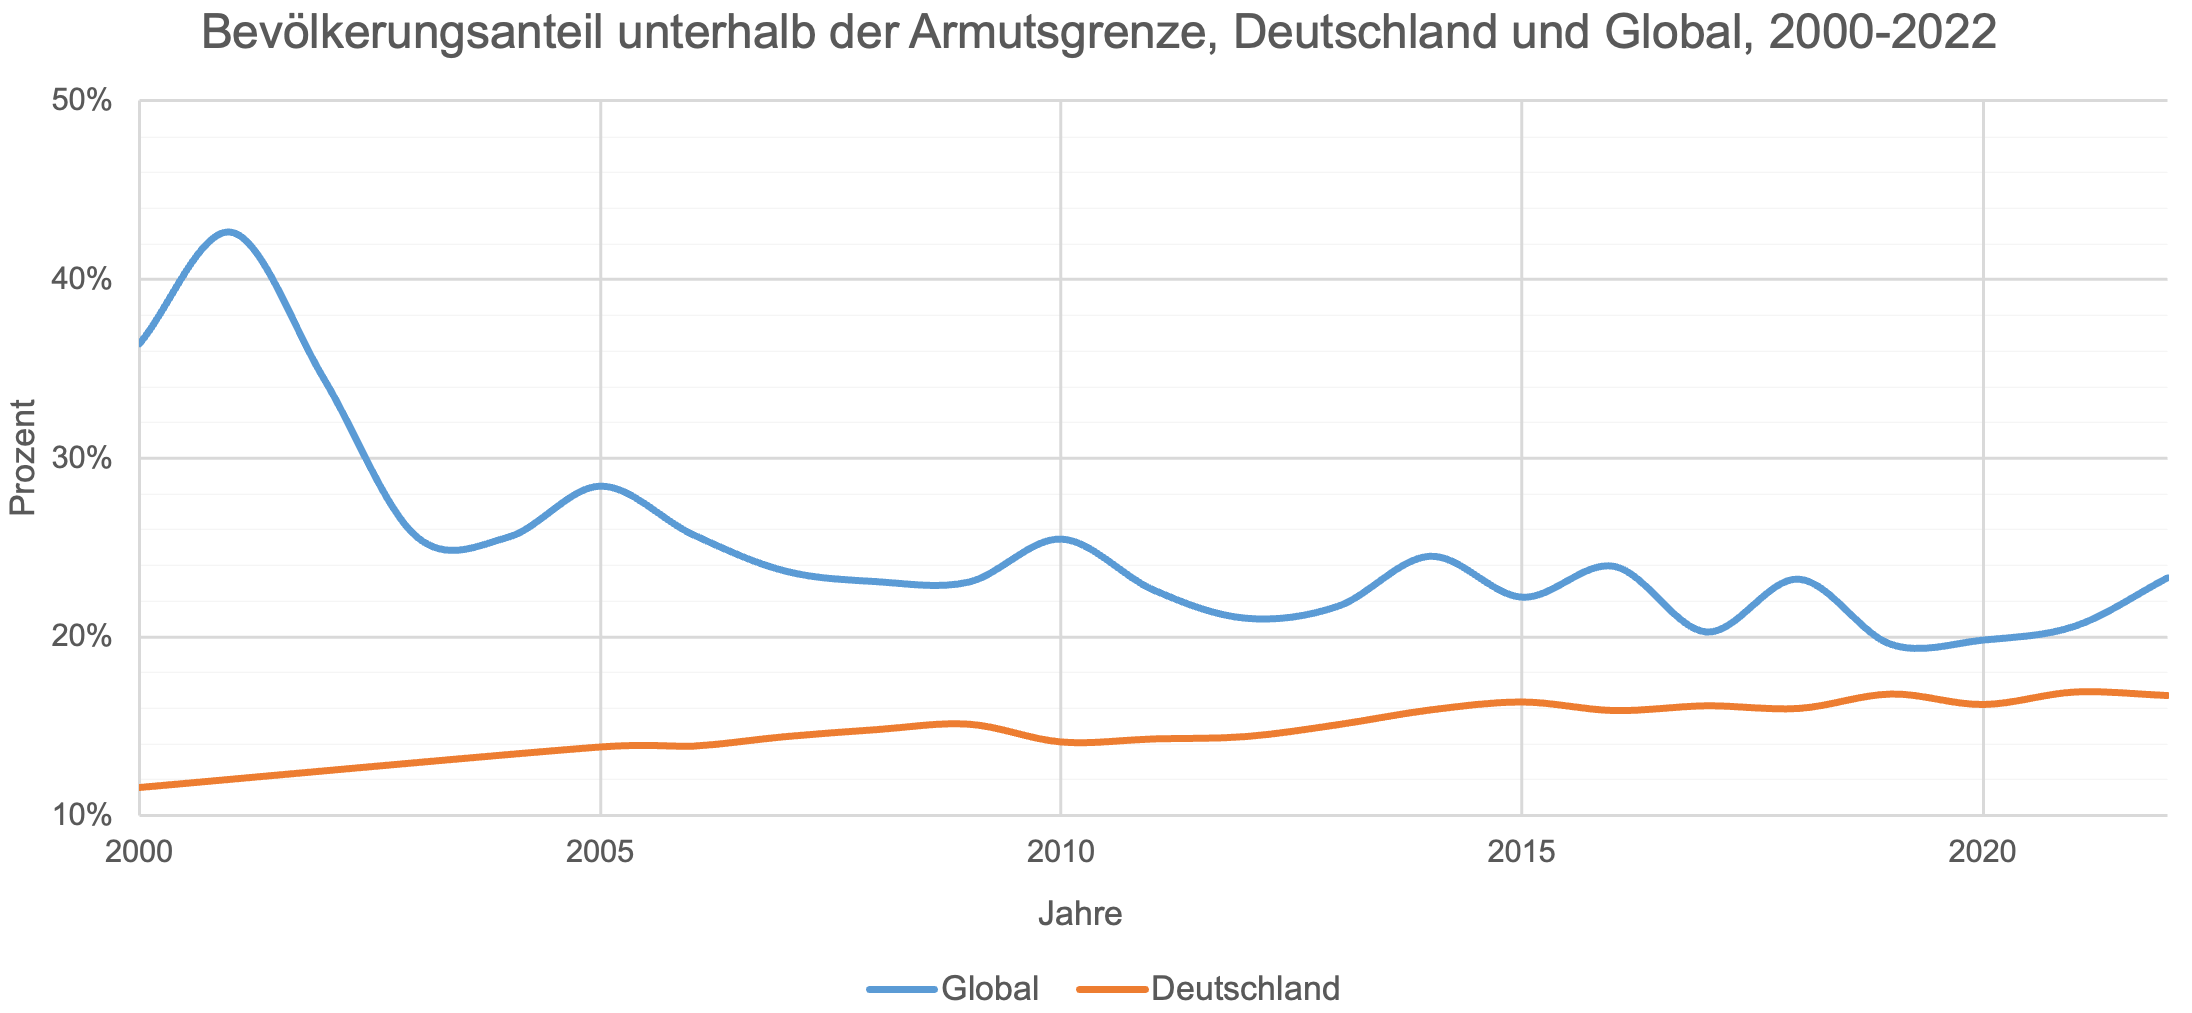
\includegraphics[height=6.9cm]{Bilder/Armutsgrenze2.png}
    \caption[Bevölkerungsanteil unterhalb der Armutsgrenze, Deutschland und global, 2000-2020]{Bevölkerungsanteil mit einem Einkommen unterhalb der Armutsgrenze in Deutschland und auf globaler Ebene von 2000 bis 2020. Eigene Darstellung und Berechnung. Daten abgerufen von \cite[][(global)]{wb_armutsquote_global_2022} und \cite[][(Deutschland)]{bmas_arb_armutsrisikoquote_2023} am 01.03.2024.}
    \label{fig:iso_norm}
\end{figure}

